% This file can be used to compile the adventure into a stand alone PDF without the sourcebook
\documentclass{book}


\usepackage{../../static/templates/fate_latex_template/fate_solarpunk}
\usepackage{montserrat}
\usepackage{ebgaramond}
\usepackage{hyperref}

%%%%%% Fixing overful hboxes
%% https://tex.stackexchange.com/questions/35/what-does-overfull-hbox-mean-why-is-there-a-black-mark-at-the-end-of-a-line
\usepackage{hyphenat}
%% \hyp{} can mark where words can break
%% Make it simpler:
%% https://tex.stackexchange.com/questions/488008/how-to-create-an-alternative-to-shortcut-or-hyp
\usepackage[english]{babel}

% Create title and background image
% https://tex.stackexchange.com/questions/136900/insert-a-full-page-image
% https://www.ctan.org/pkg/background
\usepackage[pages=some]{background}
\backgroundsetup{
scale=1,
angle=0,
opacity=1,
firstpage=true,
contents={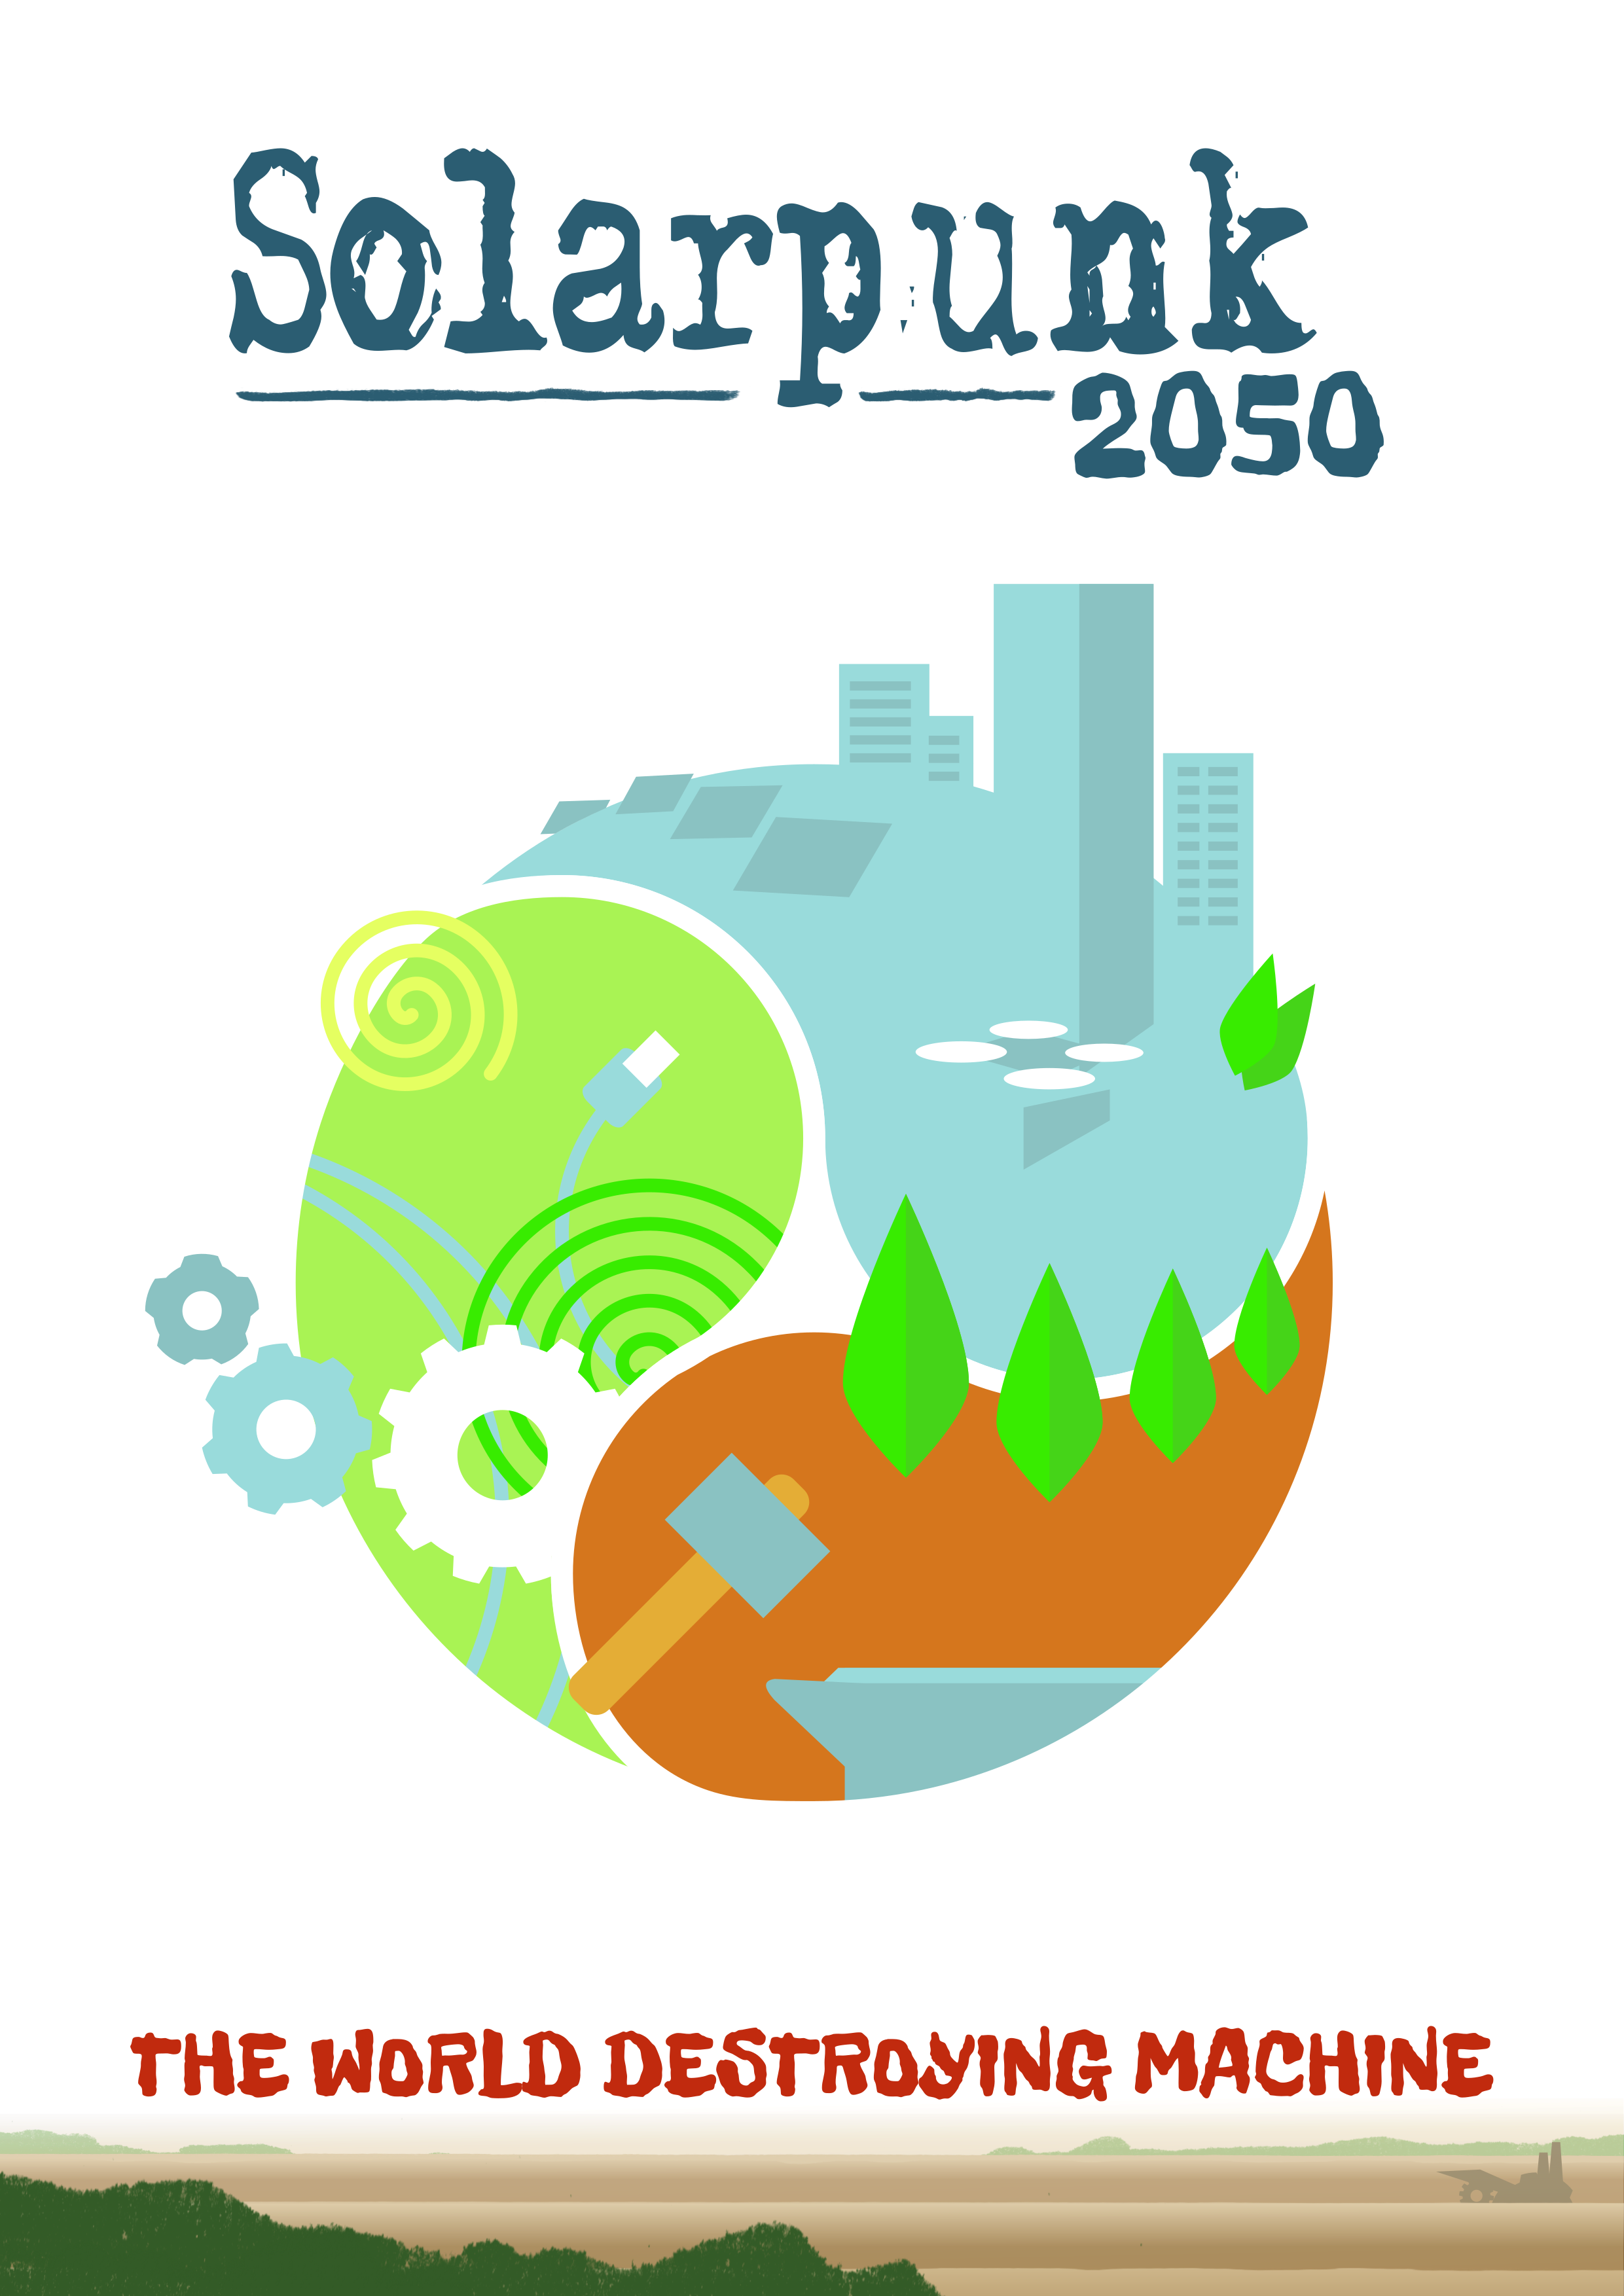
\includegraphics[width=\paperwidth,height=\paperheight]{../sourcebook/static/Solarpunk-Machine.png}}
}

\useshorthands{~}
\defineshorthand{~-}{\hyp{}}
%% ~- can mark this break now



%... other code

% \section{Hello World}
% \label{sec:hello}



% For creating example text
% \usepackage{lipsum}

\title{Fate Solarpunk 2050 - Adventure "The world destroying machine"}
\author{Thorsten Sick}

\pagenumbering{arabic}
\begin{document}

%
% Book front page
%
\mbox{}
\thispagestyle{empty}
\BgThispage


%% Hyphenation database:
\hyphenation{meal-worm Mc-Gyver fa-mous be-cause}
%%%%%

\chapter{Introduction}

Solarpunk is a utopian science fiction genre. \textbf{Solarpunk 2050} is the setting in which this goal has almost been achieved. The protagonists, called Pioneers, live in ecological, technologically advanced and socially progressive communities. Close to the big cities, where the so-called Norms go about their daily lives - pampered by their AI.

This adventure is part of the Solarpunk 2050 setting, but contains everything you need to get started - except the rules which are \href{https://fate-srd.com/fate-condensed}{Fate Condensed} and free.

\chapter{The World Destroying Machine}
\label{ch:the world destroying machine}

A simple hello-world style adventure with pre-created characters to play at cons or any time you need a short session.

Following the tradition it is a special kind of "Rats in the cellar" which seems to exist for almost all RPGs.

At this game the pre-made characters are all from the Solarpunk group. If for some reason a player can not associate with the characters available you could try to create a Lost or a Norm character and include that one. This character could be a relative of one of the Solarpunks and join the party at the beginning.

\begin{sidebarBox}[title=Dirty Road to Eden]

The people living before 2020 are called "Lemmings" in the year 2050. Named that way thanks to their self destructive habits. After 2020 more and more people doubted the wisdom of self destruction and took action. This led to a 2050 where mankind was saved and could survive in prospering automated eco-towns, Solarpunk communities and Lost camps in the middle of the wilderness and ruins of the old civilisation. But the road to this new and bright future was dirty. Not everyone could be saved. Some towns had to be sacrificed. Lots of hard decisions made fighting climate change induced disasters. 

\end{sidebarBox}

\section{Topics}

This adventure covers some typical Solarpunk topics. As a game to play with Solarpunk beginners or even Role Playing Game beginners it can be used as first steps in a tutorial.

It also offers

\begin{itemize}
\item Introduction to basics of the Solarpunk 2050 world
\item Character Interaction: Players must balance interests to earn Fate Points
\item Culture Clash: All three cultures are represented. Cooperation can be essential to success
\item The mission starts without weapons. Solarpunks can build them or get help from NPCs
\item Introducing the mistakes of the "Lemmings" (us) that lead to devastation
\end{itemize}

\section{Summary}

The map of the adventure is linear - still the protagonists can always go back and forth. To find allies, trade for tools and prepare for the last challenge.

While the the map is linear there are several options to solve the challenges which makes the adventure flexible. The player decisions and the possible solutions are sandbox-style.

The linear order is:

\begin{itemize}
\item Players get to know the Solarpunk philosophy at a Solarpunk Party in their Community
\item Task: Search the world destroying machine (=coal power plant) and recover raw materials to build a brewery
\item Protagonists meet some Lost.
\item After entering the World Destroying Machine they will meet Norms recording a series
\item The boss of this adventure has a first appearance: A mutated hamster
\item Search the World Destroying Machine, solve some problems, build weapons, deal with the hamster
\item Closing party at the construction of the brewery or dealing with the consequences of their decisions
\end{itemize}

\section{Getting Started}

\begin{sidebarBox}[title=Solarpunks]
Solarpunks are a group of hyper inventive people living in self build eco friendly high tech communities. Most of the currently used technology is based on their concepts. During the Dirty Road to Eden they have been the (uncoordinated) main driver of the revolution. Today they either do not talk about that phase or flag it as necessary to safe mankind (which it was). Most of the time they do not care about the past but focus on the future - many details have already been forgotten. Solarpunks love their creative society but are very individualistic and everyone has their own pet projects.
\end{sidebarBox}

It's a big outdoor Solarpunk party. The community has gathered. There is home made music and the usual LED and laser spectacle. Besides the normal garden grow food a special drink is served: a schnapps glass for everyone with a new beer to taste.
It is brewed with DIY gene edited yeast and a new brewing process. Delicious. And it glows thanks to bioluminescence. Unfortunately, the quantity is limited: the current laboratories and brewery devices can no longer cope. That should be expanded. And for that the community needs resource points.

\begin{sidebarBox}[title=Resource points]
\hyperref[sec:Resource points]{Resource points} are the main currency. To avoid abuse of the nature every person gets a limited amount of them each year. They are required to get any non-renewable  material based object. The ones appointed are enough for a normal life style. But not enough to build a brewery. The only way to get more of those points is by recycling objects. Big objects or those made of rare materials return more resource points. This is one of the main reasons to start an adventure visiting the ruins of the Lemmings. 
\end{sidebarBox}

By luck, a "world destroying machine" (a coal-fired power plant - but that is never mentioned) that had been buried in one of the many catastrophes was found after another flood removed half of a hill. An auction for salvage rights was started and the Solarpunks won the right to enter it first.
The party received 4 (or number of players-1) EU-issued salvage tags to stick on objects to be salvaged. Once attached, these cannot be removed without heavy equipment. The protagonists may decide what is most valuable to them. Besides the tags you can take as much as you can carry.

\begin{sidebarBox}[title=Salvage tags]
Salvage tags are sticker with small energy source and computer and radio transmitter. They become inextricably linked to an object and identify it as salvage. After the adventure, specialists (NPCs) will arrive with heavy equipment that will cut, haul, and recycle objects. And assign the points to the account of the Solarpunk community.
\end{sidebarBox}

\emph{Salvage tags are a game system to improve the game flow. This is a kind of "bag of holding". Without those tags the characters would be carrying 30 tons of power generators with them.}

% TODO: DOT graphviz goes here

\section{Party}

Topic of the scene: 
\begin{itemize}
\item Characters get to know each other
\item Players test rules
\item \bf{And especially: get a taste of the Solarpunk feeling}
\end{itemize}

The Solarpunks have an evening party outside on the community fairground. Something big is announced this time. To pass the time (and learn the rules) the protagonists can take part in one of the many activities. 
Everything is decorated with coloured lights. Scarves and pennants everywhere. People stand around in groups or dance. In the middle of the festival ground is a large pillar, the lower part of which is currently illuminated in green.
Announcement from the elders: “Today we have some news. The first: Dorothea has offspring! (Display of a video screen with live switch to a nest with chicks in the forest). <Frenetic cheers>. Quiet please! We have just put up the volume column in the centre of the festival area because of the breeding season.
It monitors the microphones distributed in the forest.
As always: If it turns red, please turn down the volume. The music systems do this automatically. This year, the Children's 5th Drone Squadron vowed to protect the clutches by keeping cats, martens and other predators out in a large perimeter around the nests. (Illuminated quadrocopters fly in formation over the festival, one of the drones quickly veers out of formation, dips elegantly into the punch bowl and immediately rejoins the formation) <Children cheer>.
The second announcement is in an hour.
"

After the first announcement the characters can entertain themselves at the party. This is to learn the rules:

\begin{itemize}
\item Juggling workshop (participation)
\item More relaxed: Gardening and chatting with the local NPCs
\item Drones race the kids around through the trees. The pilots repair broken drones themselves (participation, help with repairs, dodge drones, get them out of the trees)
\item E-motor challenge: Everyone drinks a schnapps. After that they try build a working motor from scratch (participate, medical help for drunken people)
\item Party organization: Everyone who is interested takes turns playing the music and lighting (organize music and lighting)
\end{itemize}

Just before the announcement in the evening everyone receives a shot cup of locally brewed beer. The eldest: “This beer was made with our own engineered yeast. The team around 'The Barrel' made it possible (jubilation). As you can see, the beer glows in the dark and tastes great. But without a large bio laboratory and a proper brewery, we can't produce more. . . and we lack the resource points to build one. The good news is: We have salvage rights for an ancient world-destroying machine. It was buried during a  disaster. And a new disaster just removed half of the hill above it. Let's salvage heavy machinery and rare metals, and secure resource points through recycling! That will give us our brewery laboratory!”

'The Barrel' is then allowed to answer people's most important questions during the festival: 
\begin{itemize}
\item "Does one glow after drinking ?" (No)
\item "Does the pee glow?" (Yes)
\item "How long does the pee glow?" (a few days )
\item "Can you also brew glowing lemonade for children?" (Yes)
\end{itemize}

The protagonists set off, first by train (e-bikes and quads are in the goods wagon). Then drive into a relatively new patch of forest growing on land that was flooded 20 years ago.


\section{Camp of the Lost}

Topics of the scene:

\begin{itemize}
\item You get to know the faction of the lost
\item You have the first encounter with a mutant giant hamster
\item You can acquire weapons (steal, buy)
\item One could ask the Lost for support
\end{itemize}

\begin{sidebarBox}[title=The Lost]
The Lost are survival experts, fighters and historians. They travel the country looking for ruins of "Lemmings technology" from before 2040. They reject new technology but are very skilled in reusing and upcycling old technology. Their camps look a bit ragged but are very practical. They are a bit rough compared to the "lifestyle" Norms and the "hyperactive/hypercreative" Solarpunks. When the Dirty Road to Eden started to transform the 2020 way of life into what we have now they saw that there is a high price to pay. And decided to not join that transformation out of ethical reasons.
\end{sidebarBox}

The protagonists arrive at a forest. There is a Lost camp in front of the entrance in the machine. Heavy diesel cars stand with their engines running. Oil burns in oil pans. Tents are built with old tarpaulin. Everything is makeshift built with remnants from the past. But it is practical and a decent camp.

In addition to that: A giant hamster (bear sized) on a rotisserie.

Someone is making potato salad and setting up the picnic benches. Music blares.
The speakers are misadjusted and at least 20 years old. But that doesn't bother anyone here. In the background someone is shooting at beer cans with a shotgun (this is their leader Caligula). 
The Lost got 10 salvage tags themselves in the auction. That's more than the Solarpunks have. But this is also the reason why they're second to enter the ruins. The tags are not active yet - they will be activated in 12 hours and then they can start salvaging. Until the tags are active, the Lost want to party
here in the woods. The Lost are therefore no competition if the players proceed reasonably quickly.

Behaviour: They tease the Solarpunks and ask them not to take "diesel tanks, generators or something" with
them, this technology belongs to the Lost. If the Solarpunk join the teasing and proof worthy they can get invited to a short "hamster, salad and beer".

After that's done, the Solarpunks' salvage tags activate and they're allowed to begin descending through the newly found entrance into the World Destroying Machine

\begin{npcBox}[title=Caligula]

    \begin{aspects}
    \item \aspect[High Concept]{Small budget Indiana Jones}
    \item \aspect[Trouble]{Alcohol fuelled}    
    \end{aspects}
    
    \begin{skills}
    \item \skill{4} Shoot
    \item \skill{3} Academics
    \item \skill{3} Provoke
    \end{skills}
    
    \begin{stunts}
    \item \stunt{Tuning}{Gets a +2 on shooting whenever using a gun he has recently tuned in a 1 hour practice session}
    \end{stunts}
    
    \begin{stressSection}
    \stressLine{\stress{1}\stress{1}\stress{1}}{\stress{1}\stress{1}\stress{1}}
    \end{stressSection}
    \begin{tabularx}{\textwidth}{ XX }
    \end{tabularx}
    
    \begin{consequences}
    \item \consequence{2}
    \item \consequence{4}
    \item \consequence{6}
    \end{consequences}
    
    \begin{npcDescription}
    Caligula leads a small family of ruin raiders. They travel the wildlands and look for treasure in old ruins. Whatever useful things they find they reuse in creative ways.
    He is ready to fight if he must. But would appreciate a discussion about old artefacts and sites a lot more. The first impression a stranger will see will still be the Redneck with the gun.
    \end{npcDescription}
    
    \end{npcBox}

He is not alone but his "family" is about 10 people who can use a weapon and are skilled in scouting ruins. They do not care for nature as much as the Solarpunks do. As they constantly fight and struggle with the forces of nature and the wilderness. Their approach to nature is more ... pragmatic.

If the protagonists make friends with the Lost they could gain:

\begin{itemize}
    \item Weapons and people who can use them
    \item The insight that the World Destroying machine is a coal power plant. Including a rough sketch of the map
    \item Maybe learn that Norms arrived 2 days ago. "Looked strange. But they always look strange. Not prepared for the ruins. Even less prepared than you are"
\end{itemize}

\section{Battleground}

Goal of the scene:

\begin{itemize}
\item You meet the Norms for the first time.
\item Learn: The World Destroying Machine is absurdly engineered. Almost dull and boring
\end{itemize}

\begin{sidebarBox}[title=Norms]

80 percent of the people in 2050 are Norms. They live in automated eco-towns. Governed by AIs tuning all the parameters to achieve maximum quality of life and happiness. The society is highly cooperative. Most people have a 25h/week job that is highly specialized. The AI plans projects to coordinating those specialists in a incredible dance to achieve big projects.
Norms all carry a life-logger with them. This device offers them Apps and an AR interface where they can just request things from the AI and the society. And it will be done - magic !
While the Norms enjoy their hobbies they will never achieve the solo skills Solarpunks have. They are always dependent on being close to the AI and a working society. If the requirements are not met some Apps may indicate that and will be unavailable.

Focussing on the now they do not care about the past or the Dirty Road to Eden. Everything is fine now. It must have been worth the price.

In this region all Norm characters have only limited App benefits because this region is only covered by the small AI they brought with them in a shipping container. The social network is also small. Almost everything they need will have to be delivered by drones from the next town (adding 1h). For Solarpunks this can still feel like magic.

\end{sidebarBox}

The characters enter a corridor through a crooked metal hatch at the side of a hill. After the hatch: a corridor. The walls are white - but musty now. The floor is linoleum.
White plastic cupboards devoid of any personality line the aisles. Many doors (white, plastic in wood optics) branch off to the right and left. Signs on them with the names of the people whose office this used to be. Behind the doors: rubble and mud.


Soon the protagonists will find a simulated accident. It looks realistic: A Norm actor (Delta Awesome) lies under a foam H-beam (looking like steel). A hidden cameraman (Kevin) films him screaming. Actually, the hero of the reality soap should appear at any time to 'rescue' him. Instead, the protagonists (real Solarpunks) come to the rescue.

The actor "Delta Awesome" keeps acting and "Kevin" keeps filming while the Solarpunk start the rescue. They will soon learn there was no real danger.

After the misunderstanding has been cleared up and everyone is impatiently waiting for the hero actor  "Theophil Tierlieb", you can hear some screams down the aisle. A quick look: The expected hero, actor in the role of "Theophil Tierlieb" is being pulled into a pipe by a huge bear sized hamster. These pipes seem to run through the whole World Destroying Machine.
Unfortunately, the pipe are almost impossible for a human to crawl through (being pulled unconscious by a monster seems to take up less space and the hamster itself is built for tunnels and pipes). At some point the pipe will also break due to the stress. Drones would be able to follow the beast. It is impossible to follow through the pipes. following the pipes is possible but tricky. Some of them pass through walls.

The protagonists need a map. And maybe weapons. As a Solarpunk, you improvise on the go.

At the end of the corridor, the protagonists find a large hall lined with marble. The official entrance hall and the museum of the World Destroying Machine.

\begin{npcBox}[title=Kevin\, Camera]

    \begin{aspects}
    \item \aspect[High Concept]{Camera for action}
    \item \aspect[Trouble]{Finding good action scenes}    
    \end{aspects}
    
    \begin{skills}
    \item \skill{4} Notice
    \item \skill{3} Craft (Filming)
    \item \skill{3} Empathy
    \item \skill{2} Stealth
    \end{skills}
    
    \begin{stunts}
    \item \stunt{App based Filming}{Gets a +2 on filming action scenes when in range of an AI to support him}
    \end{stunts}
    
    \begin{stressSection}
    \stressLine{\stress{1}\stress{1}\stress{1}}{\stress{1}\stress{1}\stress{1}}
    \end{stressSection}
    \begin{tabularx}{\textwidth}{ XX }
    \end{tabularx}
    
    \begin{consequences}
    \item \consequence{2}
    \item \consequence{4}
    \item \consequence{6}
    \end{consequences}
    
    \begin{npcDescription}
    Kevin loves to entertain the audience. His skills with the camera and AI based editing help him doing that. If he becomes a friend he can boost the publicity of the Solarpunk team (if they want it or not). More essential could be his Notice skills.
    "I've known I wanted to be a cameraman since the AI recommended me for the job when I was 10."


    He does not have access to weapons and can not order them by App. "Sorry, did not do the weapons tutorial yet, should I ?"

    \end{npcDescription}
    
\end{npcBox}


\begin{npcBox}[title=Delta Awesome]

    \begin{aspects}
    \item \aspect[High Concept]{Method acting actor}
    \item \aspect[Trouble]{Observe and copy the real Solarpunks}    
    \item \aspect[Aspect]{Always stay in character}    
    \end{aspects}
    
    \begin{skills}
    \item \skill{4} Craft (Acting)
    \item \skill{3} Contacts
    \item \skill{3} Rapport
    \item \skill{2} Deception
    \item \skill{2} Athletics
    \end{skills}
    
    \begin{stunts}
    \item \stunt{Acting}{Can use Craft/Acting to convince people to join his heroic mission}
    \end{stunts}
    
    \begin{stressSection}
    \stressLine{\stress{1}\stress{1}\stress{1}}{\stress{1}\stress{1}\stress{1}}
    \end{stressSection}
    \begin{tabularx}{\textwidth}{ XX }
    \end{tabularx}
    
    \begin{consequences}
    \item \consequence{2}
    \item \consequence{4}
    \item \consequence{6}
    \end{consequences}
    
    \begin{npcDescription}
    Delta Awesome is the actor's role name. His role is that of a skilled Solarpunk expert. But he
    does not do justice to this. Since he insists on method acting and has to stay in role (otherwise it will take 2 hours until he adjusts again). He will also constantly try to improve the role by observing and copying the Solarpunks.
    
    Delta Awesome's equipment is useless tool props. In the film they are always exactly the ones he needs. 

    For his role he trained and got some real muscles. Which can be convenient. This and his acting/charisma fuelled skill to convince people to help. But to benefit from that he will have to be convinced first.
    \end{npcDescription}
    
\end{npcBox}


\section{Exhibition}

Topics of the scene:
\begin{itemize}
\item First clear indications of coal power (when researching the exhibition)
\item Socialize with the Norms
\item Find out where the pipes lead (on models and plans)
\item You can find many kilograms of protein paste here
\end{itemize}


The camera man Kevin and Delta Awesome quickly lead the protagonists to the "headquarters". A former museum (also a film location). Here catering is set up. The Norms plan to accommodate 500 fans of the series there after filming finishes. With 10 extra seats for VIPs. The party location is currently prepared.

There is an old museum in which school classes could learn something about coal power from very beautiful models.
Everything is done nicely. With a mascot. Also interesting is the mineral collection, with a huge geode, which might interest Disco.

At the catering there is a food designer (Cherie) who makes real-looking mealworms out of protein paste for the Solarpunk food shots.  That way the VIPs can feel like solar punks but don't have to eat mealworms.
The paste is made from mealworms. It's just not clear to them - but it says on the packaging.

The food designed can App-control a 3D food printer and could also fabricate a protein based fake body to trap the hamster with.

According to the food designer, the others are deeper into the World Destroying Machine to set it up for filming. Haven't heard from them in a while. (Info: They were hoarded). Access is through a steel door which is closed.

Someone with historical knowledge (Books) can figure out that the heaviest part here is probably the coal plant generator with flywheel. This can be found deeper in the plant.

Cherie has a key for the door leading deeper into the plant. It could be stolen or she could be persuaded.The lock could also be picked or the door weld open.


\begin{npcBox}[title=Cherie]

    \begin{aspects}
    \item \aspect[High Concept]{Food artist}
    \item \aspect[Trouble]{Want to be my friend ?}    
    \item \aspect[Aspect]{Food must be tasty and beautiful}    
    \end{aspects}
    
    \begin{skills}
    \item \skill{4} Craft (Food artist)
    \item \skill{3} Rapport
    \item \skill{3} Notice    
    \end{skills}
    
    \begin{stunts}
    \item \stunt{Acting}{Can use Craft/Acting to convince people to join his heroic mission}
    \end{stunts}
    
    \begin{stressSection}
    \stressLine{\stress{1}\stress{1}\stress{1}}{\stress{1}\stress{1}\stress{1}}
    \end{stressSection}
    \begin{tabularx}{\textwidth}{ XX }
    \end{tabularx}
    
    \begin{consequences}
    \item \consequence{2}
    \item \consequence{4}
    \item \consequence{6}
    \end{consequences}
    
    \begin{npcDescription}
    Does catering and simulates a Solarpunk world for spectators and guests.
    
    She loves to chat while working and is positive and cheerful. A challenge like "build a body with your 3D printer and protein" would be accepted with glee.

    Maybe that could distract the hamster ?

    The monster next door worries her a lot because she grew up in a very safe environment - a Norm town.

    \end{npcDescription}
    
\end{npcBox}



\section{Coal Bunker}

Topics of the scene:
\begin{itemize}
\item Overcome technical problems
\item Can build weapons
\item Show dirtiness of World Destroying Machine
\end{itemize}

Problems:

\begin{itemize}
\item Dry coal dust (explosive)
\item Dark black water below, with oil film
\item The norms built the SFX stuff. In particular, cables through the water and prepared pyrotechnics
\item Some of the old processes still seem to be running. The norms have been wildly hooking up batteries and motors in hopes of bringing things to life. Looks good on film but could be a death trap.
\end{itemize}

Weapon Material:

\begin{itemize}
\item Coal dust (potato cannon, pipe bombs)
\item pipes from handrails
\item explosives from the SFX
\end{itemize}

Following a dirty corridor, the protagonists enter a huge hall. Coal wagons full of coal were delivered here on rails. Some of them are still there. Derailed and crushed by the catastrophe that happened many years ago. Here the coal was checked for quality, ground to pellets and dust, transported by belts down the hall. Much of this can still be seen here - but in a sad state.
Everything is massively rusted. The coal dust hangs in the air (and is explosive !). There are black puddles on the floor (oil and coal).
At least it's clear where the Norms went. They left behind batteries, lights and pyrotechnics and their trail runs diagonally through the area. This obstacle course could blow up at any time. Careful navigation, some parcours, engineering to cut through metal and defusing explosives are required. Lots of skill throws.

The conveyor belt for the coal leads to the next room where the protagonists will want to go.


\section{Walkways}

Topics of the scene:
\begin{itemize}
\item Overcome obstacles
\item Demonstrate the desolation and grandeur of the world-destroying machine
\item Can build weapons
\end{itemize}

The protagonists will have to climb over catwalks and through big running ventilation fans.
Those are spooky backlit and a fog machine makes an eerie optics. The SFX people have been here. I'm sure it looks great in the movie.
Greenish glowing dust puffs (mutated) grow on the ground below. Someone with eco knowledge would know that the spores are psychoactive. The director lies slurring by the mushrooms.
A make-up opportunity is set up below. The shooting here is already planned.

Problems:
\begin{itemize}
\item Broken metal walkways
\item Pipe labyrinths (in which hamsters move)
\item Mutated mushrooms, the director must be rescued 
\end{itemize}

Weapon material:

\begin{itemize}
\item Sharp blades from ventilation (Swords)
\item Pieces of pipe (spears, pipe bomb, potato cannon)
\item Psychoactive mushrooms (wear protective gear when harvesting !)
\end{itemize}


The conveyor belt leads to the combustion chamber ( which is not accessible). Next door is the generator room. There is the nest.
In this room you can already see steam pipes that lead there.

\begin{npcBox}[title=Lucien\, Director]

    \begin{aspects}
    \item \aspect[High Concept]{Film director with a skill for blockbusters}
    \item \aspect[Trouble]{There is a story in there}    
    \end{aspects}
    
    \begin{skills}
    \item \skill{4} Craft (Film director)
    \item \skill{3} Contacts
    \item \skill{3} Resources
    \end{skills}
    
    \begin{stressSection}
    \stressLine{\stress{1}\stress{1}\stress{1}}{\stress{1}\stress{1}\stress{1}}
    \end{stressSection}
    \begin{tabularx}{\textwidth}{ XX }
    \end{tabularx}
    
    \begin{consequences}
    \item \consequence{2}
    \item \consequence{4}
    \item \consequence{6}
    \end{consequences}
    
    \begin{npcDescription}
    Is stoned when found and will not recover before the end of the story. Could be interesting as a friend at the Party.s
    \end{npcDescription}
    
\end{npcBox}

\section{Nest}

Topics of the scene:
\begin{itemize}
\item Final Battle
\end{itemize}

All kinds of organic material can be found in the nest. Ranging from old sacks of potatoes to dead animals (hunted dogs and wild boars).
It's confusing and full of debris from ancient civilization.
The hamster himself dragged the lifeless Norm onto the heap and he will die here soon.
A special treasure here are the 4 large generators with the heavy, massive flywheel. This is the treasure that could be tagged for salvage (either after the hamster is dead or by sneaking in). 

Solution ideas:
\begin{itemize}
\item You could make the hamster overeat with fake protein so that she falls asleep (Bio
Knowledge to trigger the "eat now" reflex)
\item Or intoxicate her with the psychoactive mushrooms (Bio Skills, Weapon Technique)
\item Or kill her (combat)
\item Or fetch the Lost for help (Social Interaction)
\item Sneak in and rescue the injured, also secretly attaching salvage tags
\item Dazzle the hamster by drones, pyro, SFX...
\end{itemize}


\begin{npcBox}[title=Hamster]

    \begin{aspects}
    \item \aspect[High Concept]{Fluffy killer machine on a CCS mission}
    \item \aspect[Trouble]{Damned by the genes}
    \item \aspect[Aspect]{Always hungry for protein}
    \end{aspects}
    
    \begin{skills}
    \item \skill{4} Power
    \item \skill{3} Fight
    \item \skill{3} Notice
    \end{skills}
    
    \begin{stunts}
    \item \stunt{Through the pipes}{Using \bf{notice} the hamster can enter a pipe and emerge 1 round later at a tactical spot anywhere else in the room gaining an advantage for the attack (+2). By being better at \bf{notice} the player characters can find out where the hamster is moving and negate the effect.}
    \end{stunts}
    
    \begin{stressSection}
    \stressLine{\stress{1}\stress{1}\stress{1}\stress{1}\stress{1}\stress{1}}{\stress{1}\stress{1}\stress{1}}
    \end{stressSection}
    \begin{tabularx}{\textwidth}{ XX }
    \end{tabularx}
    
    \begin{consequences}
    \item \consequence{2}
    \item \consequence{4}
    \item \consequence{6}
    \end{consequences}
    
    \begin{npcDescription}
    The hamster is bear sized and when attacked can be quite aggressive. Her normal goal is to harvest proteins and drag them down here. Storing them. When searching the protagonists can also find out: The hamster is female and has 4 young hamsters in a nest she is protecting.
    \end{npcDescription}
    
\end{npcBox}


\begin{npcBox}[title=Theophil Tierlieb]

    \begin{aspects}
    \item \aspect[High Concept]{Actor in role of "Theophil Tierlieb" - animal whisperer}
    \item \aspect[Trouble]{Animals hate the real me}
    \item \aspect[Aspect]{Hamster chow}
    \end{aspects}
    
    \begin{skills}
    \item \skill{4} Craft (Acting)
    \item \skill{3} Contacts
    \item \skill{3} Charisma
    \end{skills}
        
    \begin{stressSection}
    \stressLine{\markedstress{1}\markedstress{1}\markedstress{1}}{\stress{1}\stress{1}\stress{1}}
    \end{stressSection}
    \begin{tabularx}{\textwidth}{ XX }
    \end{tabularx}
    
    \begin{consequences}
    \item \consequence{2} Headache
    \item \consequence{4} Broken bones
    \item \consequence{6} Strong bleeding
    \end{consequences}
    
    \begin{npcDescription}
    Playing a animal whisperer but learning after 2 episodes that animals hate him he continued suffering for 3 seasons until attack by a real monster hamster. But the audience loves his role.
    \end{npcDescription}
    
\end{npcBox}


\section{The real end boss}

After the fight the protagonists will find 4 tiny monster hamsters (tiny = the size of a dog). The kids of the mother they just killed. They are old enough to survive without mother if someone cares for them. They did not attack people. But could do that in the future. Now it is up to the protagonists to decide:

\begin{itemize}
    \item Take them to the Community and care for them ?
    \item Kill them
    \item Leave them to their fate ?
    \item Sell them to the Lost (so they can be fattened and later be slaughtered) ?
\end{itemize}

You see, the real end boss is a dilemma and you should make it extra dramatic. Trigger a 5 minute discussion between the characters if possible to find the best way. Make it clear that earned resource point could not be enough for a monster hamster cage and a brewery.

\section{Victory Party}

Topics:

\begin{itemize}
\item Serves to conclude the adventure and to celebrate.
\item Shows the consequences of their decisions
\end{itemize}

A few days later. The resource points were exchanged for raw materials. Those arrived at the Community and a brewery can be built. Building it is part of a party with music, food and drinks.

Friends they made will be invited. They will play a role in the celebration.

If they rescued the tiny monster hamster they will have to build a giant hamster cage first. Including a wheel and pipes crossing through the Community. Maybe the resource points will not be enough for brewery and cage ?

\section{Player characters}

\begin{itemize}
\item Books: Scholar, wants to salvage historical things
\item Curly: Acrobat, wants to recover something funny
\item The Barrel: Brewer, wants to salvage objects as large as possible because of raw material points - the brewery wants them
\item Disco: Bard, wants to salvage beautiful things
\item Spark: Tech, wants to recover technology
\item Primrose: Ecology, wants to save nature
\end{itemize}

%%%%%%%%%% Books

\begin{npcBox}[title=Books]

    \begin{aspects}
    \item \aspect[High Concept]{Scholar - think first then act}
    \item \aspect[Trouble]{We don't do anything without a plan}
    \item \aspect[Relationship]{I wrote an article, could you please review it ?}    
    \item \aspect[Aspect]{The more I know the better I perform}        
    \end{aspects}
    
    \begin{skills}
    \item \skill{4} Academics
    \item \skill{3} Notice
    \item \skill{3} Investigate
    \item \skill{2} Athletics
    \item \skill{2} Rapport   
    \item \skill{2} Fight
    \item \skill{1} Drive
    \item \skill{1} Crafts
    \item \skill{1} Shoot
    \item \skill{1} Will

    \end{skills}
    
    \begin{stunts}
    \item \stunt{E-Book}{Whuile I have my treasured e-book, I get +2 when I use Academics}
    \end{stunts}
    
    \begin{stressSection}
    \stressLine{\stress{1}\stress{1}\stress{1}}{\stress{1}\stress{1}\stress{1}\stress{1}}
    \end{stressSection}
    \begin{tabularx}{\textwidth}{ XX }
    \end{tabularx}
    
    \begin{consequences}
    \item \consequence{2}
    \item \consequence{4}
    \item \consequence{6}
    \end{consequences}
    
    \begin{npcDescription}
    Hunter for knowledge. Wearing a jacket with patches on the elbows. Hair is turning grey.
    \end{npcDescription}


    \begin{equipment}
    \item Light source (OLED film: battery operation, can be cut to size and glued on. Colour controllable)
    \item Food (Mama Salsa's Famous Mealworm Buns in the Bento Box)
    \item First aid kit
    \item Mobile computers, headphones, communication via radio (mesh network)
    \end{equipment}
    
\end{npcBox}

%%%%%%%%%%% Curly

\begin{npcBox}[title=Curly]

    \begin{aspects}
    \item \aspect[High Concept]{Childish climbing acrobat}
    \item \aspect[Trouble]{Secret fan of bad Norm TV series}
    \item \aspect[Relationship]{Always looks for a role model in the group}    
    \item \aspect[Aspect]{Let's see if I can do something fun with it. . .}        
    \end{aspects}
    
    \begin{skills}
    \item \skill{4} Athletics
    \item \skill{3} Stealth
    \item \skill{3} Fight
    \item \skill{2} Burglary
    \item \skill{2} Notice  
    \item \skill{2} Deceive
    \item \skill{1} Shoot
    \item \skill{1} Rapport
    \item \skill{1} Craft
    \item \skill{1} Power

    \end{skills}
    
    \begin{stunts}
    \item \stunt{E-Tail}{With my furry balance tail, I get +2 on Acrobatics when balancing}
    \end{stunts}
    
    \begin{stressSection}
    \stressLine{\stress{1}\stress{1}\stress{1}\stress{1}}{\stress{1}\stress{1}\stress{1}}
    \end{stressSection}
    \begin{tabularx}{\textwidth}{ XX }
    \end{tabularx}
    
    \begin{consequences}
    \item \consequence{2}
    \item \consequence{4}
    \item \consequence{6}
    \end{consequences}
\end{npcBox}
\newpage
\begin{npcBox}[title=Curly continued]
    \begin{npcDescription}
    Clean-shaven head, a scale pattern tattooed. Wearing a self-made balance suit (with balancing tail).        
    \end{npcDescription}


    \begin{equipment}
    \item Light source (OLED film: battery operation, can be cut to size and glued on. Colour controllable)
    \item Food (Mama Salsa's Famous Mealworm Buns in the Bento Box)
    \item First aid kit
    \item Mobile computers, headphones, communication via radio (mesh network)
    \item A stripped down light exoskeleton with a balancing tail
    \item Climbing rope
    \end{equipment}
\end{npcBox}


%%%%%%% The Barrel


\begin{npcBox}[title=The Barrel]

    \begin{aspects}
    \item \aspect[High Concept]{Strong listener}
    \item \aspect[Trouble]{Likes to talk to microorganisms (yeasts)}
    \item \aspect[Relationship]{Active counseling. "How are you with that?"}    
    \item \aspect[Aspect]{Driving force of the beer project}        
    \end{aspects}
    
    \begin{skills}
    \item \skill{4} Empathy
    \item \skill{3} Academic (genetics)
    \item \skill{3} Craft (brewing)
    \item \skill{2} Power
    \item \skill{2} Fight  
    \item \skill{2} Notice
    \item \skill{1} Rapport
    \item \skill{1} Drive
    \item \skill{1} Athletics
    \item \skill{1} Will

    \end{skills}
    
    \begin{stunts}
    \item \stunt{Empathy}{Because I'm highly empathic, using empathy to help someone gives me a +2. Unfortunately, his problems won't let me go for
    some time.}
    \end{stunts}
    
    \begin{stressSection}
    \stressLine{\stress{1}\stress{1}\stress{1}\stress{1}}{\stress{1}\stress{1}\stress{1}\stress{1}}
    \end{stressSection}
    \begin{tabularx}{\textwidth}{ XX }
    \end{tabularx}
    
    \begin{consequences}
    \item \consequence{2}
    \item \consequence{4}
    \item \consequence{6}
    \end{consequences}
\end{npcBox}
\newpage
\begin{npcBox}[title=The Barrel continued]
    \begin{npcDescription}
    Comfortable, bearish, strong. Interested in optimizing the art of brewing and ready to read up on genetic engineering.
    \end{npcDescription}


    \begin{equipment}
    \item Light source (OLED film: battery operation, can be cut to size and glued on. Colour controllable)
    \item Food (Mama Salsa's Famous Mealworm Buns in the Bento Box)
    \item First aid kit
    \item Mobile computers, headphones, communication via radio (mesh network)
    \item Gene laboratory in a suitcase
    \item 2 bottles of glowing beer (prototype)
    \end{equipment}
\end{npcBox}


%%%%%%%% Disco

\begin{npcBox}[title=Disco]

    \begin{aspects}
    \item \aspect[High Concept]{Fighter for the colourful lights and the eternal party}
    \item \aspect[Trouble]{Discomfort in serious situations}
    \item \aspect[Relationship]{wants everyone to be happy and get along}
    \item \aspect[Aspect]{Searching for beautiful things}        
    \end{aspects}
    
    \begin{skills}
    \item \skill{4} Rapport
    \item \skill{3} Empathy
    \item \skill{3} Craft (SFX)
    \item \skill{2} Contacts
    \item \skill{2} Shoot
    \item \skill{2} Notice
    \item \skill{1} Athletics
    \item \skill{1} Drive
    \item \skill{1} Power
    \item \skill{1} Deception

    \end{skills}
    
    \begin{stunts}
    \item \stunt{Disco !}{Because I'm Disco Artist, I get +2 when I use Craft (SFX) to draw or manipulate attention or mood of people or creatures using my disco systems.}
    \end{stunts}
    
    \begin{stressSection}
    \stressLine{\stress{1}\stress{1}\stress{1}\stress{1}}{\stress{1}\stress{1}\stress{1}}
    \end{stressSection}
    \begin{tabularx}{\textwidth}{ XX }
    \end{tabularx}
    
    \begin{consequences}
    \item \consequence{2}
    \item \consequence{4}
    \item \consequence{6}
    \end{consequences}
\end{npcBox}
\newpage
\begin{npcBox}[title=Disco continued]
    \begin{npcDescription}
    Fidgety colourful party kid. Clothing has expanded over the years to include more and more quirky accessories
    \end{npcDescription}


    \begin{equipment}
    \item Light source (OLED film: battery operation, can be cut to size and glued on. Colour controllable)
    \item Food (Mama Salsa's Famous Mealworm Buns in the Bento Box)
    \item First aid kit
    \item Mobile computers, headphones, communication via radio (mesh network)
    \item A dozen mini lighting drones for festivals
    \item Disco sound equipment (loudspeakers, recordings, microphones, all wirelessly connected)
    \end{equipment}
\end{npcBox}

%%%%%%%%% Primrose

\begin{npcBox}[title=Primrose]

    \begin{aspects}
    \item \aspect[High Concept]{Lovable and pacifistic eco-terrorist}
    \item \aspect[Trouble]{Nature gets by best without people}
    \item \aspect[Relationship]{Nature is great. People are ok too.}
    \item \aspect[Aspect]{Find new nature and preserve it}        
    \end{aspects}
    
    \begin{skills}
    \item \skill{4} Academics (Biology and Ecology)
    \item \skill{3} Athletics
    \item \skill{3} Stealth
    \item \skill{2} Rapport
    \item \skill{2} Burglary
    \item \skill{2} Crafts (Explosives)
    \item \skill{1} Empathy
    \item \skill{1} Deception
    \item \skill{1} Notice
    \item \skill{1} Will

    \end{skills}
    
    \begin{stunts}
    \item \stunt{Do Drugs}{Because I'm experienced Eco-Terroristy, I get +2 when I use Academics (Biology) to use psychoactive substances to manipulate moods.}
    \end{stunts}
    
    \begin{stressSection}
    \stressLine{\stress{1}\stress{1}\stress{1}}{\stress{1}\stress{1}\stress{1}\stress{1}}
    \end{stressSection}
    \begin{tabularx}{\textwidth}{ XX }
    \end{tabularx}
    
    \begin{consequences}
    \item \consequence{2}
    \item \consequence{4}
    \item \consequence{6}
    \end{consequences}
\end{npcBox}
\newpage
\begin{npcBox}[title=Primrose continued]
    \begin{npcDescription}
    Cloths are visible eco textiles - something that is not necessary with today's technology. It is a conscious decision.
    \end{npcDescription}


    \begin{equipment}
    \item Light source (OLED film: battery operation, can be cut to size and glued on. Colour controllable)
    \item Food (Mama Salsa's Famous Mealworm Buns in the Bento Box)
    \item First aid kit
    \item Mobile computers, headphones, communication via radio (mesh network)
    \item Lock picking set
    \item Little biolab in a box
    \end{equipment}
\end{npcBox}


%%%%%%%% Spark

\begin{npcBox}[title=Spark]

    \begin{aspects}
    \item \aspect[High Concept]{A punk in action - with tools}
    \item \aspect[Trouble]{Wants to learn new tricks from old technology}
    \item \aspect[Relationship]{Motivate others to tinker}
    \item \aspect[Aspect]{If it's small: shake it, if it's big: kick it}        
    \end{aspects}
    
    \begin{skills}
    \item \skill{4} Craft
    \item \skill{3} Academics (Engineering)
    \item \skill{3} Power
    \item \skill{2} Fight
    \item \skill{2} Drive
    \item \skill{2} Resources
    \item \skill{1} Athletics
    \item \skill{1} Shoot
    \item \skill{1} Notice
    \item \skill{1} Will

    \end{skills}
    
    \begin{stunts}
    \item \stunt{McGyver genes}{Because I have McGyver gear and genes, I get +2 when I use crafting to screw something together in a hurry. Immediately after the successful use of the improvised hack it will probably fail spectacularly.}
    \end{stunts}
    
    \begin{stressSection}
    \stressLine{\stress{1}\stress{1}\stress{1}\stress{1}\stress{1}\stress{1}}{\stress{1}\stress{1}\stress{1}\stress{1}}
    \end{stressSection}
    \begin{tabularx}{\textwidth}{ XX }
    \end{tabularx}
    
    \begin{consequences}
    \item \consequence{2}
    \item \consequence{4}
    \item \consequence{6}
    \end{consequences}
\end{npcBox}
\newpage
\begin{npcBox}[title=Spark continued]
    \begin{npcDescription}
    "Straw hat" plaited from scraps of cable, other pieces of machinery woven into clothes.
    \end{npcDescription}


    \begin{equipment}
    \item Light source (OLED film: battery operation, can be cut to size and glued on. Colour controllable)
    \item Food (Mama Salsa's Famous Mealworm Buns in the Bento Box)
    \item First aid kit
    \item Mobile computers, headphones, communication via radio (mesh network)
    \item Laser welder (no weapon)
    \item Duct tape, WD40 and Swiss army knife
    \end{equipment}
\end{npcBox}

%% A small world description specifically for this adventure.
%% It is compiled in instead of the large variant when the text is compiled as quickstart

\chapter{Small world description}

Some guides for the GM

\section{Pioneers}
\label{sec:Pioneers}
Guide to playing Pioneers: They are always busy with some project or other. They will tell you about it and try to recruit you. Either that, or they will throw the most absurd party ever. This drive can also be destructive, and accidents are quite common in a Pioneer society. But the experience of dealing with laboratory accidents has also grown.
Make it fun and dynamic.
They stretch towards the future like leaves towards the sun.

\section{Lost}
\label{sec:Lost}
Guide to playing Lost: This group is deeply rooted in the past. They distrust high tech (basically anything with a microcontroller). You will find survivalists, militaristic types, farmers and craftsmen. But their treasures are things from the past. Especially books.
First and second contact will be with simple people who have the thick skin and survival instincts to deal with whatever nature throws at them. Stay longer with the Lost and you may meet some of the wise and well-read.


\section{Norms}
\label{sec:Norms}
Guide to playing Norms: Norms live in the present. They are always connected to each other, and cooperative thinking is their typical mode of operation. They are also connected to their hive (in this case a distant city) and the Core AI.
It is quite common for a norm to try to reach a consensus before acting.
Living in a post-scarcity economy, most of them are busy producing art and entertainment. Or soap operas. Living in shelter, it is hard for them to accept a harsh reality.


\section{Resource points}
\label{sec:Resource Points}
In the post scarcity world the resource points are the only thing limited. Those represent damage to the nature like burning fossil fuel or using non-renewable resources. For you as GM: Make it the most valuable resource and use it as a carrot.

\chapter{Solarpunk 2050}



\end{document}